%source mathadata
\begin{multicols}{2}
			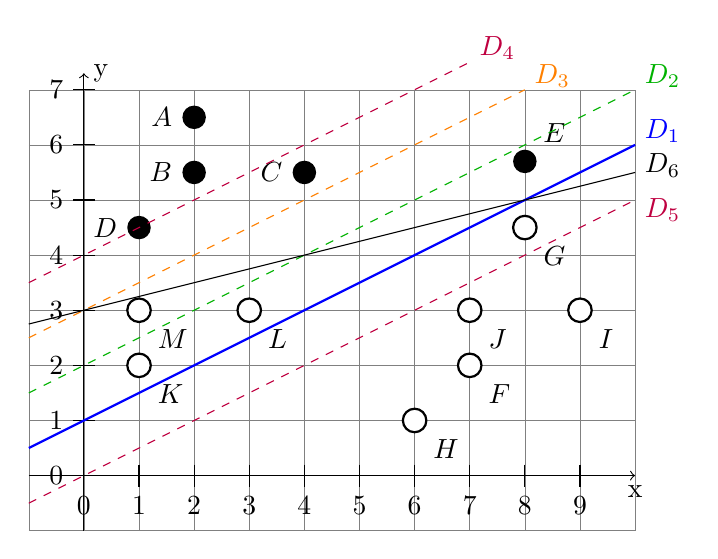
\begin{tikzpicture}[scale=0.7]
				\tikzset{
					grid major/.style = {very thin, gray},
					grid minor/.style = {very thin, lightgray}
				}
				\draw[grid major] (-1, -1) grid[step=1] (10, 7);
				\draw[->] (-1,0) -- (10,0) node[below] {x};
				\draw[->] (0,-1) -- (0,7.3) node[right] {y};
				\foreach \x in {0,1,...,9} \draw (\x,0.2) -- (\x,-0.2) node[below] {\x};
				\foreach \y in {0,1,...,7} \draw (0.2,\y) -- (-0.2,\y) node[left] {\y};
				\node at (2,6.5) [circle,fill,inner sep=3pt,label=left:{$A$}] {};
				\node at (2,5.5) [circle,fill,inner sep=3pt,label=left:{$B$}] {};
				\node at (4,5.5) [circle,fill,inner sep=3pt,label=left:{$C$}] {};
				\node at (1,4.5) [circle,fill,inner sep=3pt,label=left:{$D$}] {};
				\node at (8,5.7) [circle,fill,inner sep=3pt,label=above right:{$E$}] {};
				\node at (7,2) [circle,fill=white,thick,draw,inner sep=3pt,label=below right:{$F$}] {};
				\node at (8,4.5) [circle,fill=white,thick,draw,inner sep=3pt,label=below right:{$G$}] {};
				\node at (6,1) [circle,fill=white,thick,draw,inner sep=3pt,label=below right:{$H$}] {};
				\node at (9,3) [circle,fill=white,thick,draw,inner sep=3pt,label=below right:{$I$}] {};
				\node at (7,3) [circle,fill=white,thick,draw,inner sep=3pt,label=below right:{$J$}] {};
				\node at (1,2) [circle,fill=white,thick,draw,inner sep=3pt,label=below right:{$K$}] {};
				\node at (3,3) [circle,fill=white,thick,draw,inner sep=3pt,label=below right:{$L$}] {};
				\node at (1,3) [circle,fill=white,thick,draw,inner sep=3pt,label=below right:{$M$}] {};

				% Droites parallèles
				\draw[domain=-1:10, smooth, variable=\x, blue, thick] plot ({\x}, {0.5*\x+1});
				\node[font=\bfseries, blue] at ({10.5}, {0.5*10.5+1}) {$D_1$};

				\draw[domain=-1:10, smooth, variable=\x, green!70!black, dashed] plot ({\x}, {0.5*\x+2});
				\node[font=\bfseries, green!70!black] at ({10.5}, {0.5*10.5+2}) {$D_2$};

				\draw[domain=-1:8, smooth, variable=\x, orange, dashed] plot ({\x}, {0.5*\x+3});
				\node[font=\bfseries, orange] at ({8.5}, {0.5*8.5+3}) {$D_3$};

				\draw[domain=-1:7, smooth, variable=\x, purple, dashed] plot ({\x}, {0.5*\x+4});
				\node[font=\bfseries, purple] at ({7.5}, {0.5*7.5+4}) {$D_4$};

				\draw[domain=-1:10, smooth, variable=\x, purple, dashed] plot ({\x}, {0.5*\x});
				\node[below=1pt, font=\bfseries, purple] at ({10.5}, {0.5*10.5}) {$D_5$};

				% Droite D6
				\draw[domain=-1:10, smooth, variable=\x] plot ({\x}, {0.25*\x+3});
				\node[font=\bfseries] at ({10.5}, {0.25*10.5+3}) {$D_6$};
			\end{tikzpicture}

			\begin{MADenumerate}
				\item $\boldsymbol{y = 0{,}5x + 1}$

				\item
				\begin{enumerate}
					\item 4 erreurs : $G$, $K$, $L$, $M$
					\item Pourcentage d'erreur : $\dfrac{4}{13} \approx 30{,}8\%$
				\end{enumerate}

				\item
				\begin{enumerate}
					\item Voir graphique.
					\item $D_2$ : 2 erreurs ($E$, $M$).

					      Pourcentage d'erreur : $\dfrac{2}{13} \approx 15{,}4\%$
					\item Exemples :

					      $D_3 : y = 0{,}5x + 3$ → 1 erreur ($E$) → $ 7{,}7\%$

					      $D_4 : y = 0{,}5x + 4$ → 2 erreurs ($C$, $E$) → $15{,}4\%$

					      $D_5 : y = 0{,}5x + 0$ → 4 erreurs ($G$, $K$, $L$, $M$) → $38{,}5\%$

				\end{enumerate}

				\item $D_3$ a le plus faible pourcentage d'erreur : $7{,}7\%$ (1 erreur sur 13).

				\item Pour $W(2;3{,}5)$ avec $D_3$ : $$y = 0{,}5\times 2 + 3 = 4.$$

				Comme $3{,}5 < 4$, $W$ est en dessous de $D_3$ donc c'est un \textbf{point noir} pour cette droite.

				\item La droite $D_6$ passant par les points $(0;3)$ et $(8;5)$ d'équation $y = 0{,}25x + 3$ sépare parfaitement les points blancs et les points noirs avec un pourcentage d'erreur de $0\%$.
			\end{MADenumerate}
		\end{multicols}
